% Chapter 1

\chapter{Driving signals} % Main chapter title
\label{Ch:signals} % For referencing the chapter elsewhere, use \ref{Chapter1} 

The complex networks grow through the addition of new nodes, and growing networks models consider that growth is constant over time. This approximation is sufficient for explaining how properties of complex networks can emerge; for example, in the Barabasi-Albert model such as in real systems, we find scaling of degree distribution. Models mostly focus on linking rules and their influence on the topology of complex networks. 

Still, the growth of real systems changes over time. In online social networks, new users join on daily basis and the users' activity might have bursty nature. We can consider a co-authorship network, where links are created between scientists when they publish a paper. The dynamic of real networks can be complex and highly influenced by non-linear signals. The growth signal; the number of new nodes in each time step; has cycles and trends. Circadian cycles are directly reflected into growth signals and we also find long-range correlations and multifractal properties. 

In this chapter, we explain the properties of growth signals, both real and computer-generated. We analyze networks created with a growing network model where the interplay between ageing and preferential attachment shape their structure. We are interested to incorporate non-constant growth signals into the model and measure their impact on the complex networks. Differences between networks with the same number of nodes and links can be observed through connectivity patterns. Figure \ref{fig:ciljevi} describe used model. 
   

\begin{figure}[!ht]
	\centering
	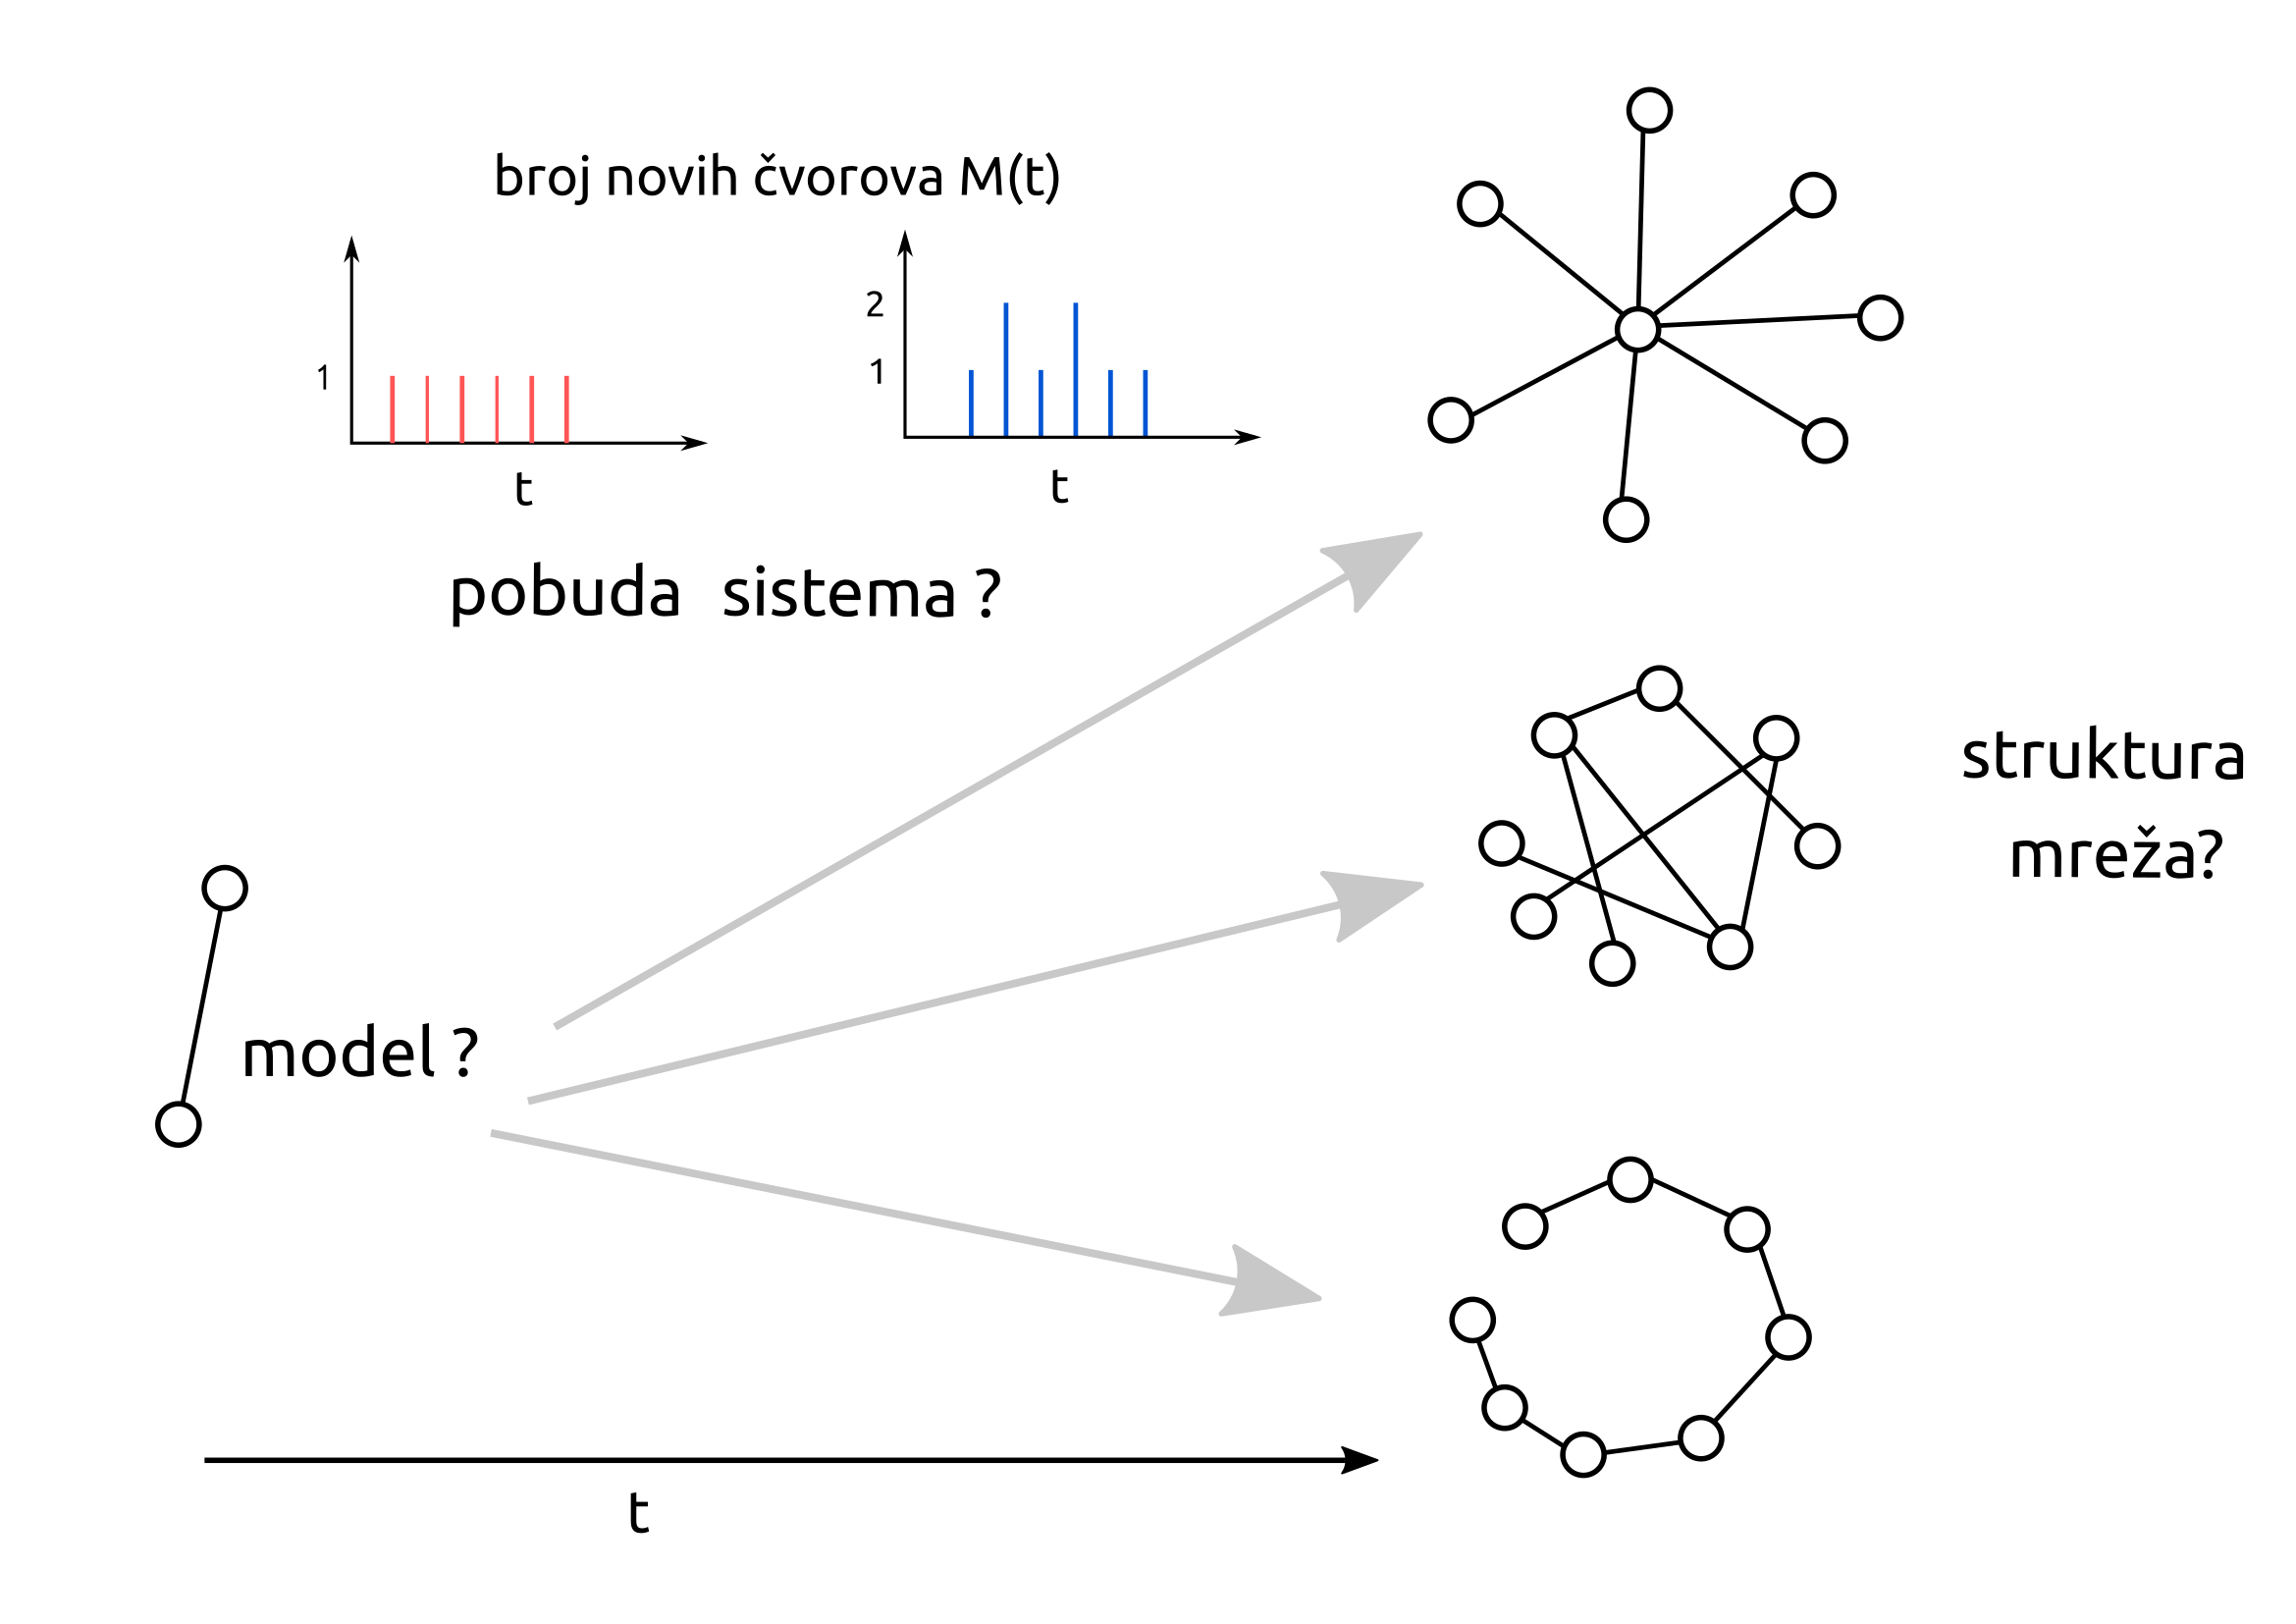
\includegraphics[width=0.6\linewidth]{Figures/ciljevi3.png}
	\caption{Growing network model schema.}
	\label{fig:ciljevi}
\end{figure}

\section{Growing signals}

\subsection{Long range correlated signals}

The main characteristic of long-range correlated time series is power law decay of autocorrelaction function, $C(s)= <x_i x_{i+1}> = s ^ {-\delta}$. Instead of using correlation function to directly determine type correlations in the signal, in practice is more common to calculate Hurst exponent.  

Hurst exponent is used for estimating self-similarity of the time series described with relation $x(ct)=cHx(t)$. Hurst exponent and autocorrelation coefficient $\delta$ are connected  as  $H = 1- \frac{\delta}{2}$. When $H=0.5$ signal has short range correlations and is considered to be white noise, while for $H=1.0$ signal is pink noise. Between this limits $0.5<H<1.0$, signal has long range correlations.

Monofractal signals can be generated using Fourier transform method \cite{makse1996method}:
\begin{itemize}
	\item first generate one-dimensional sequence of uncorrelated random numbers $u_i$ from Gaussian distribution with $\sigma=1$
	\item calculate the Fourier transform of the generated sequence, $u_q$
	\item filter signal $x_q = u_q s$, where $s$ is Fourier transform of autocorrelation function $C(s)$ 
	\item the inverse Fourier transform $x_i$ is signal with specific long range correlations 
\end{itemize}     

\begin{figure}[h!]
	\centering
	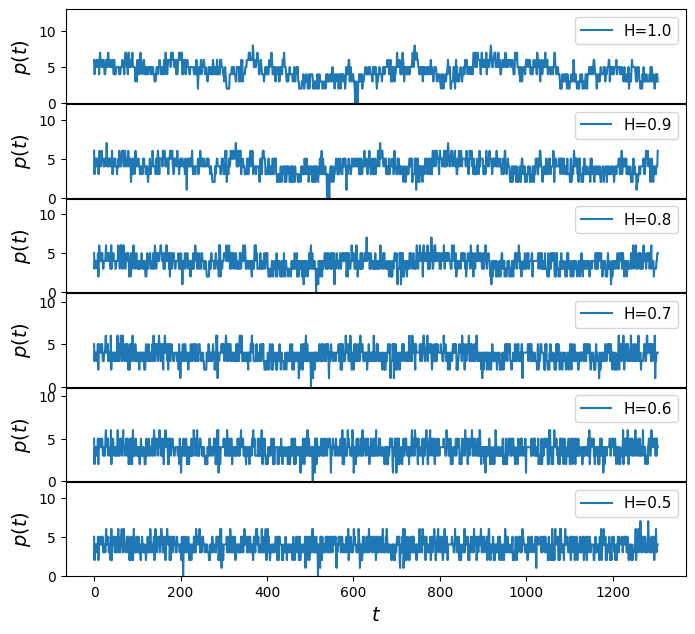
\includegraphics[width=0.7\linewidth]{Figures/monofractals.png}
	
	\caption{Monofractal signals}\label{fig:monofractals}
\end{figure}

Figure \ref{fig:monofractals} shows artificial signals generated using Fourier transform method for different values of Hurst exponents. The obtained signals are round to integers, as in real time series integer values are present. The mean values of signals are close to $4$.

For estimation of Hurst exponent from non-stationary signal can be used detrended fluctuation analasys (DFA) \cite{kantelhardt2001} \cite{peng1994}. This method removes trends and cycles from the signal, while Hurst exponent is estimated based on residual fluctuations. Signals from real world have usually  multifractal structure and can not be described with only one value of Hurst exponent \cite{kantelhardt2002}.



\subsection{Real signals}

In this work, we use two different growth signals from real systems figure 1: (a) the
data set from TECH community from Meetup social website [36] and (b) two months
dataset of MySpace social network [37]. TECH is an event-based community where
members organize offline events through the Meetup site [36]. The time unit for TECH
is event since links are created only during offline group meetings. The growth signal
is the number of people that attend the group’s meetings for the first time. MySpace
signal shows the number of new members occurring for the first time in the dataset [37]
with a time resolution of one minute. The number of newly added nodes for the TECH
signal is N = 3217, and the length of the signal is T = 3162 steps. We have shortened
the MySpace signal to T = 20221 time steps to obtain the network with N = 10000
nodes.
\begin{figure}[!ht]
	\centering
	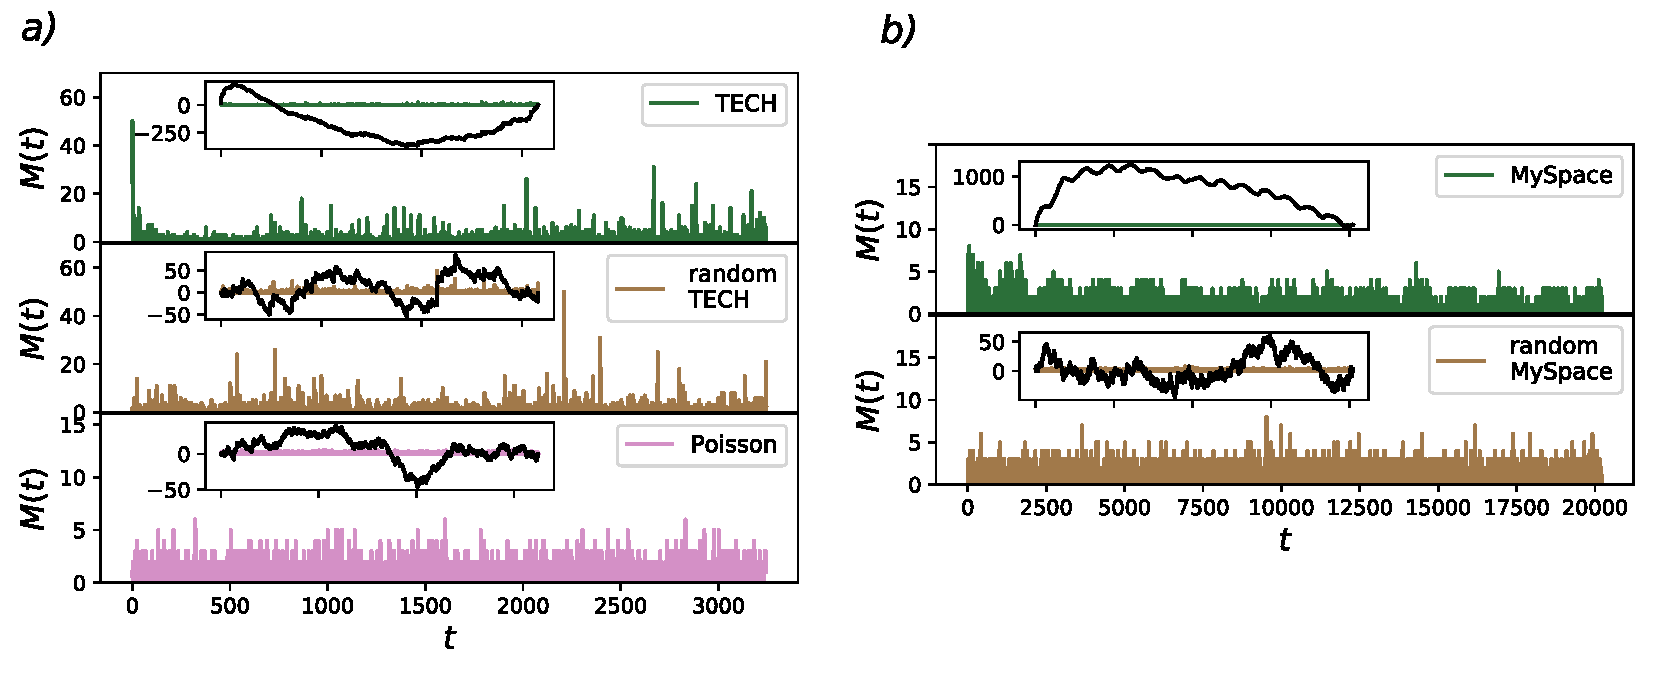
\includegraphics[width=\linewidth]{Figures/signals.pdf}
	\caption{Growth signals for TECH (a) and MySpace (b) social groups, their randomized counterparts, and random signal drawn from Poasonian distribution with mean $1$. The cumulative signals are shown in insets.}
	\label{fig:signals}
\end{figure}

\begin{figure}[!ht]
	\centering
	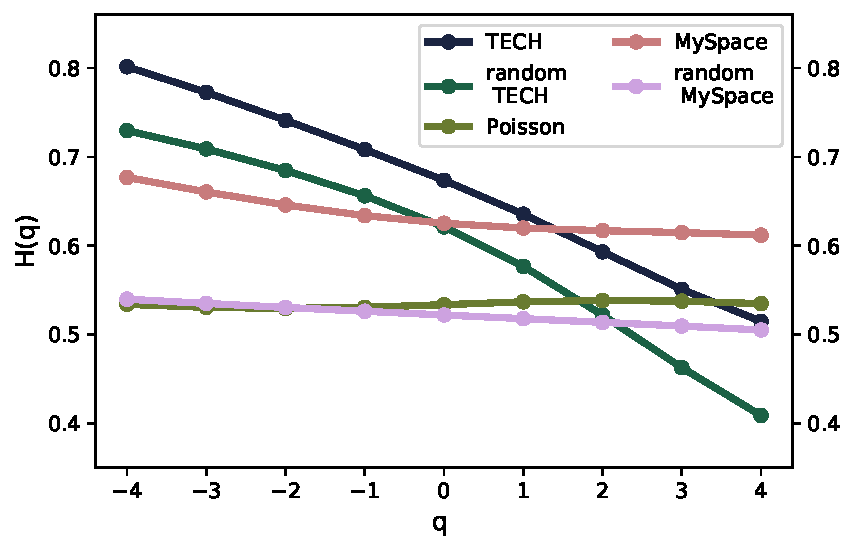
\includegraphics[width=0.6\linewidth]{Figures/hurst.pdf}
	\caption{Dependence of Hurst exponent on parameter $q$ for all five signals shown in figure \ref{fig:signals} obtained with MFDFA. }
	\label{fig:mfdfa}
\end{figure}
Real growth signals have long-range correlations, trends and cycles [37, 27, 25]. We
also generate networks using randomized signals and one computer-generated white-
noise signal to explore the influence of these signal’s features on the structure of
evolving networks. We randomize real signals using reshuffling procedure and keep their
length and mean value, the number of added nodes, and probability density function
of fluctuations intact, but destroy cycles, trends, and long-range correlations. Besides,
we generate a white-noise signal from a Poissonian probability distribution with a mean
equal to 1. The length of the signal is T = 3246, and the number of added nodes in the
final network is the same as for the TECH signal.

Figures \ref{fig:signals} (a) and \ref{fig:mfdfa} show that the TECH signal has long trends and a broad probability density function of fluctuations. The trends are erased from the randomized TECH signal, but the broad distribution of the signal and average value remain intact. MFDFA analysis shows that real signals have long-range correlations with Hurst exponent approximately $0.6$ for $q=2$, figure \ref{fig:mfdfa}. The TECH signal is multifractal, the consequence of both broad probability distribution for the values of time series and different long-range correlations of the intervals with small and large fluctuations. Shuffling of the time series does not destroy the broad distribution of values, the reason for the persistent multifractality of the TECH randomized signal, figure \ref{fig:mfdfa}.

MySpace signal has a long trend with additional cycles that are a consequence of human circadian rhythm, figure \ref{fig:signals}(b). It is multifractal for $q<0$, and has constant value of $H(q)$ for $q>0$, figure \ref{fig:mfdfa}. In MFDFA, with negative values of $q$, we put more emphasis on segments with smaller fluctuations, while for positive $q$ emphasis is more on segments with larger fluctuations \cite{ihlen2012}. Segments with smaller fluctuations have more persistent long-range correlations in both real signals, see figure \ref{fig:mfdfa}. Randomized MySpace signal and Poissonian signal are monofractal and have short-range with $H=0.5$ correlations typically for white noise.    


\section{Growing network model with aging nodes}


The networks generated with constant growth signal are uncorrelated trees. 

To enable formation of clusters in the network new nodes need to create more than one link. We adapt the original model such that at each time step we add $M\geq1$ new nodes that make $L\geq1$ links with existing nodes in the network corresponding to probability \ref{eq:1}. 
The master equation for $N_k$, $k$ degree nodes can be written as:

\begin{equation}
\partial_{t}N_{k}=\sum^{M(t)}_{j=1}r_{k-j\longrightarrow k}N_{k-j}-\sum^{M(t)}_{j=1}r_{k\longrightarrow k+j}N_{k}+M(t)\delta_{k,L} . \label{eq:aging_master}  
\end{equation}

At each time step we add $M(t)$ nodes with $L$ links. As multiply links between two nodes are not allowed, we'll get $M(t)$ new nodes with degree $L$, that describes third term in the equation. Old nodes can increase their degree from 1 to $M(t)$, as same node can be chosen by different new nodes. The first term in the equation describes nodes with degree $k\in\{k-M(t),\ldots, k-1\}$ that getting degree $k$, while in second term nodes with degree $k$ entering degree  $k\in\{k+1,\ldots, k+M(t)\}$. The quantities $r_{k-j\longrightarrow k}$ and $r_{k\longrightarrow k+j}$ are the rates that express the transitions of a node from class with degree $k-j$ to one with degree $k$ and from class with degree $k$ to class with degree $k+j$ respectively. 

The equation \ref{eq:aging_master} is not solvable in a general case. It was solved for the case $M(t)=1$ and specific values of parameters $\alpha$ and $\beta$ using continuous approach \cite{dorogovtsev2001b}. In this work, we use numerical simulations to explore the case when $M(t)$ is a correlated time-varying function and study how these properties influence the structure of generated networks for different values of parameter $-\infty<\alpha\leq-1$ and $\beta\geq1$ and constant $L$.


\section{Structural differences between networks }

The advantage this measure has is that it can distinguish between networks generated with the same model parameters. To examine how different growth signals influence the network structure, we use D-measure and compare networks generated with the same model parameters $\alpha$, $\beta$ and fixed number of links per new node $L$, but different growth signals. The growth of first network is driven by fluctuating signal $M_1 = {M(t)}$, while the other one grows by constant rate $M_2=<M(t)> = const$. 

We focus on the region of model phase diagram with negative $\alpha$ and positive $\beta$ as there is found the transition line from stretched-exponential across scale-free to the small world- gel networks. We take range of parameters  $-3\leq\alpha\leq-0.5$ and $1\leq\beta\leq3$ with steps $0.5$ and we also vary the the number of links each new node can create $L\in{1, 2, 3}$. For each combination of $(\alpha, \beta, L)$ we generate the sample of $100$ networks, and compare the structure of network grown with fluctuating and the constant signal. The results represented by D-measure are obtained averaging the D-measure between all possible pairs of generated networks.     

\begin{figure}[h!]
	\centering
	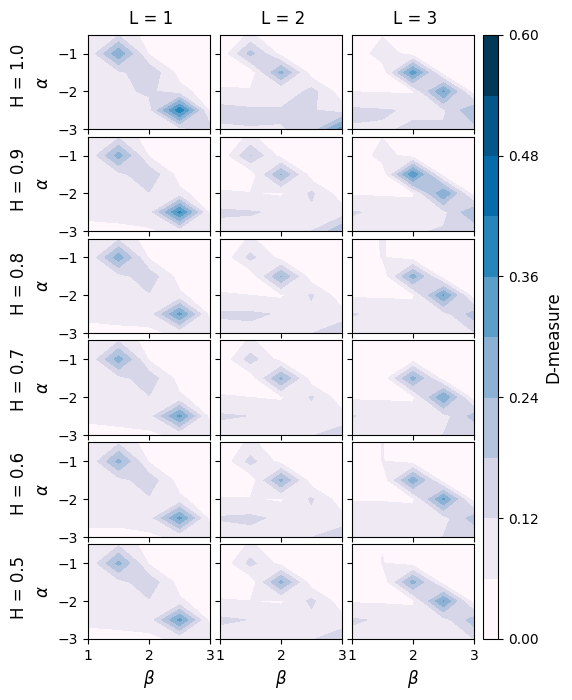
\includegraphics[width=0.5\textwidth]{Figures/Ddist_M4_w10.5_w20.5.png}
	\caption{D-distance between networks generated with different long-range correlated signals with fixed value of Hurst exponent and networks generated with constant signal M=4.}
	\label{fig:Ddist_m}
\end{figure}

First, we explore how monofractal signals, see Figure \ref{fig:monofractals} shape the structure of complex networks. The D-measure between networks grown with monofractal signal, with $H \in \{0.5, 0.6, 0.7, 0.8, 0.9, 1.0\}$ and constant signal $M=4$ are shown in figure \ref{fig:Ddist_m}. The higher values of D-measure are found in the region of critical line $\beta(\alpha^{*})$. The most considerable influence is on networks with scale-free distribution. Comparing D-distance in only one point of  phase diagram, for example $L=1, \alpha = -2.5, \beta = 2.5$, we find correlations in the signal (Hurst exponent is larger), make bigger impact on the network structure. D-measure between networks grown with signal with Hurst exponent $H=1.0$ and constant signal is $D(H=1.0, M=4) = 0.405$, while between networks grown with signal with $H=0.8$ and constant signal is $D(H=0.8, M=4) = 0.316$. For $\alpha>\alpha^{*}$ networks have similar structural properties and D-measure is close to 0. In the region of networks with stretched exponential degree distribution $\alpha<\alpha^{*}$  differences are small.  

For signals from real communities we find non-zero values of D-measure \ref{fig:dmeasure}. The largest difference between networks is as before along critical line $\beta(\alpha^{*})$, for scale free network. For values $\beta<\beta(\alpha^{*})$ the structural differences exist, but they become smaller. In the region of gel small world networks $\alpha>\alpha^{*}$ structural differences are small and close to zero. In the region around critical line we find that D-measure depends on the properties of the signal. Multifractal signals TECH has the largest impact on network structure; the maximum obtained value of D-measure is $D_{max}=0.552$. Similar behavior we discover for other multifractal signals, random TECH and MySpace. For networks generated with uncorelated signals, random mySpace and Poisson, difference exists but it is much smaller and comparable with monofractal signals.  


\begin{figure}[h!]
	\centering
	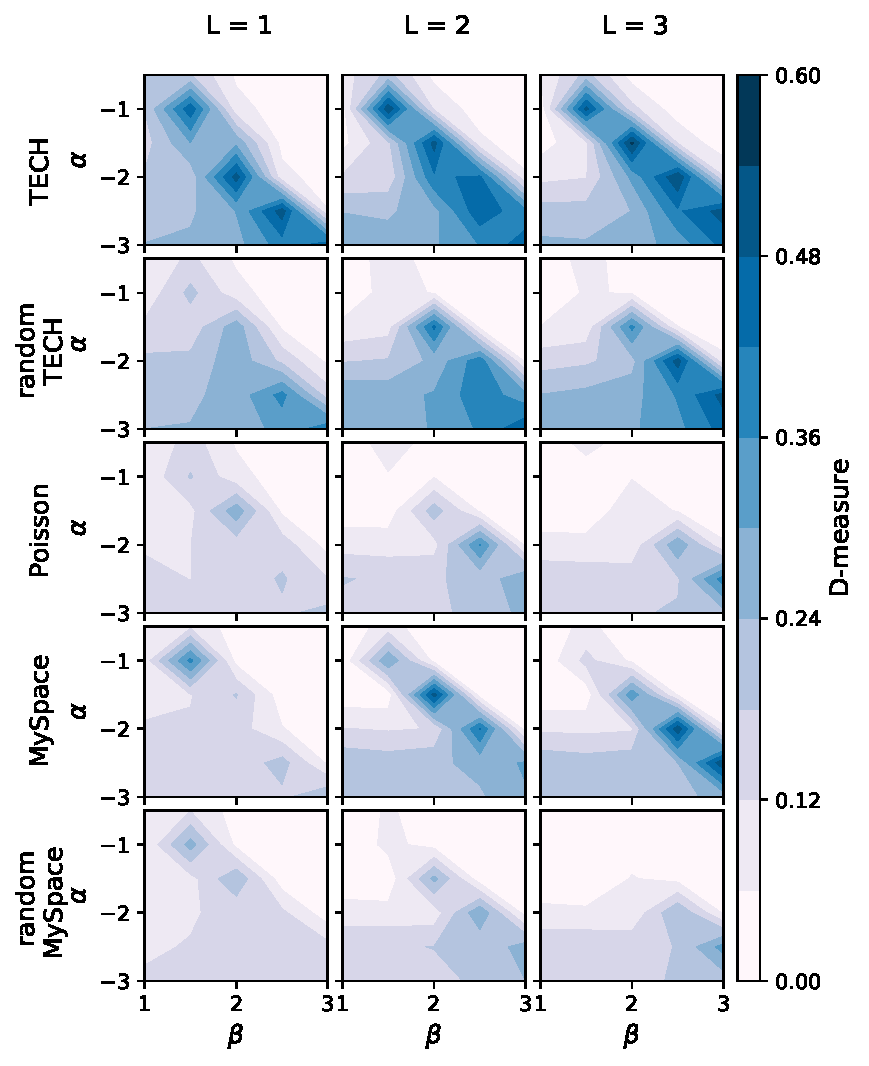
\includegraphics[width=0.5\linewidth]{Figures/Ddistance.pdf}
	\caption{The comparison of networks grown with growth signals shown in figure \ref{fig:signals} versus ones grown with constant signal $M=1$, for value of parameter $\alpha\in[-3,-1]$ and $\beta\in[1,3]$. $M(t)$ is the number of new nodes, and $L$ is the number of links added to the network in each time step. The compared networks are of the same size.}
	\label{fig:dmeasure}
\end{figure}

The position of the critical line slightly moves toward larger $\beta$ with higher link density $L$. The addition of more than one node does not influence its position. Although, for fixed network density, we find a critical line independent of the growth signal's properties as can be seen in Figures \ref{fig:dmeasure}, \ref{fig:Ddist_m}. 

We can note that D-measure rises for lower $\alpha$. In the case of constant signal, number of nodes added to the network is equal for each time step, so at time interval $T$ the network has $MT$ nodes. In fluctuating signal the number of nodes  added during time interval $T$ vary with time. In signals, such as TECH, where are present peaks in the number of new users, emergence of hubs happens faster. As we decrease the parameter $\alpha$, fluctuations present in the signal become more important and emergence of the hubs happens even for uncorrelated signals. The trends present in the real signals further promote the emergence of hubs in the network.    

\subsection{The assortativity and clustering}

We further explore the assortativity index and clustering coefficient of networks generated with monofractal signals with different values of Hurst exponent. We show results for several ageing model parameters to show the difference between network this model can produce, \ref{fig:aindex}. All networks are disassortative, with a negative degree-degree correlation index. For the values of parameters below critical line, $\alpha=-2.5, \beta=1.5$ $r$ does not depend on the Hurst exponent. Above the critical line are small-world networks, and they are disassortative with a minimum value of assortativity index $r =-1$, for $L=1$, indicating the presence of a hub that connects to many nodes. The assortativity index slightly grows with link density. 

In the region of critical parameters, the assortativity index depends on the value of the Hurst exponent. The larger influence on the assortativity index have correlated signals, with Hurst exponent $H>0.8$, so networks become more disassortative, see line for parameters $L=1, \alpha=-2.5, \beta=2.5$ in Figure \ref{fig:aindex}. The long-range correlations have a stronger effect on the evolution of networks with lower density. 

We calculate the mean clustering coefficient, Figure \ref{fig:aindex}. For $L=1$ networks are uncorrelated trees, with clustering coefficient $0$. For network density $L>1$, nodes are organized into clusters. Under the critical line, for parameter  $L=3, \alpha=-2.5, \beta=1.5 $, clustering coefficient is constant and low. Similar values are obtained for clustering coefficient for critical parameters $L=3, \alpha=-1.5, \beta=2.0$, but for Hurst exponent $H>0.8$ clustering coefficient increase. Small world networks,  $L=3, \alpha=-1.5, \beta=2.5$ are clustered, the value of $<c>$ is high.  The value of clustering for networks created with the constant signal is 0.8. Networks grown with white noise signal and signal with H=0.6 have higher values of the clustering, while networks grown with signals that have Hurst exponent larger than 0.6 have the same value of clustering, which is below 0.8. 
 
\begin{figure}[h!]
	\centering
	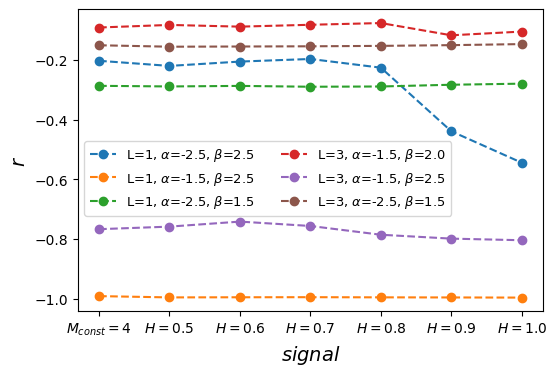
\includegraphics[width=0.45\textwidth]{Figures/aindex.png}
	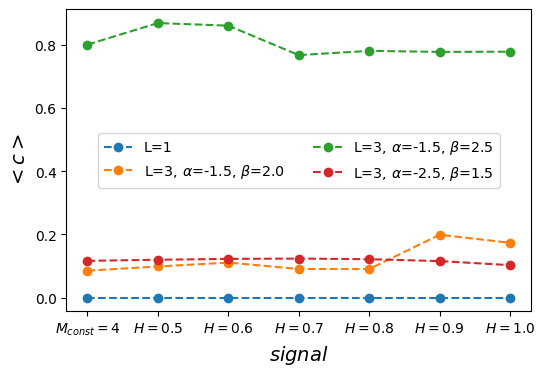
\includegraphics[width=0.45\textwidth]{Figures/clustering.png}
	\caption{Aindex}
	\label{fig:aindex}
\end{figure} 

We examine degree distribution, degree correlations and clustering coefficient of networks generated by real signals, as researchers has shown that these measures provide the sufficient set for discribing structure of complex network. D-measure showed that multifractals have larger influence on networks than monofractals, especially on scale-free networks. 

Figure \ref{fig:properties_sf} shows properties of networks generated with model parameters $L=2$, $\alpha=-1.0$, $\beta=1.5$, that lies on critical line.  The degree distributions $P(k)$ of networks generated with real signals TECH and MySpace have emergence of super-hubs. Degree distributions generated with randomized signals and white noise signal do not differ from degree distribution of networks generated with constant signal. Networks generated with real signals average neighbouring degree $\langle k\rangle_{nn}(k)$ and clustering coefficient $c(k)$ depend on node degree, while in networks generated with constant and randomized signals they weakly depend on the degree $k$.

\begin{figure}[h!]
	\centering
	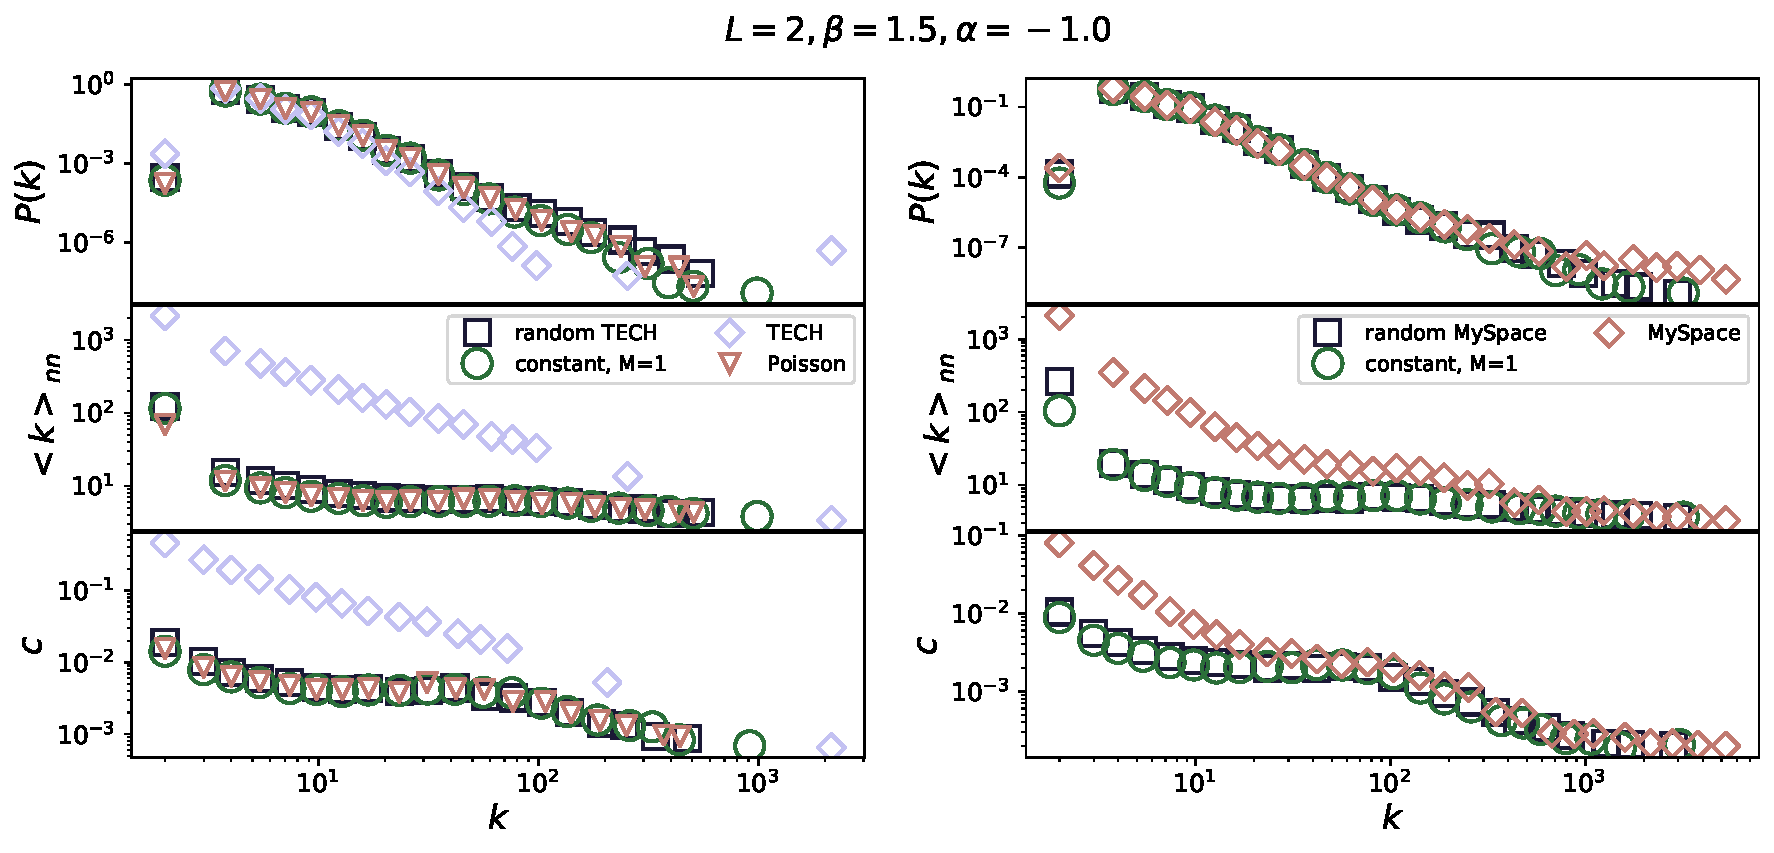
\includegraphics[width=0.7\textwidth]{Figures/b1.pdf}
	\caption{Degree distribution, the dependence of average first neighbor degree on node degree, dependence of node clustering on node degree for networks grown with different time-varying and constant signals. Model parameters have value $\alpha=-1.0$, $\beta=1.5$  and $L=2$ for all networks. The networks are from scale-free class.}
	\label{fig:properties_sf}
\end{figure}

We also find structural differences between networks, obtained with model parameters under the critical line $\alpha<\alpha^{*}$, see Figure \ref{fig:properties_se}. The difference is mostly found for TECH signal. Degree distribution $P(k)$ shows emergence of hubs in networks grown with TECH signal, while the randomized and Poisson signal are more similar to networks grown with constant signal. MySpace signal; whose generalized Hurst exponent $H(q)$ weakly depends on scale parameter $q$ and whose long-range correlations and trends are easily destroyed; do not influence the structure of networks more than constant or randomized signal.   

\begin{figure}[h!]
	\centering
	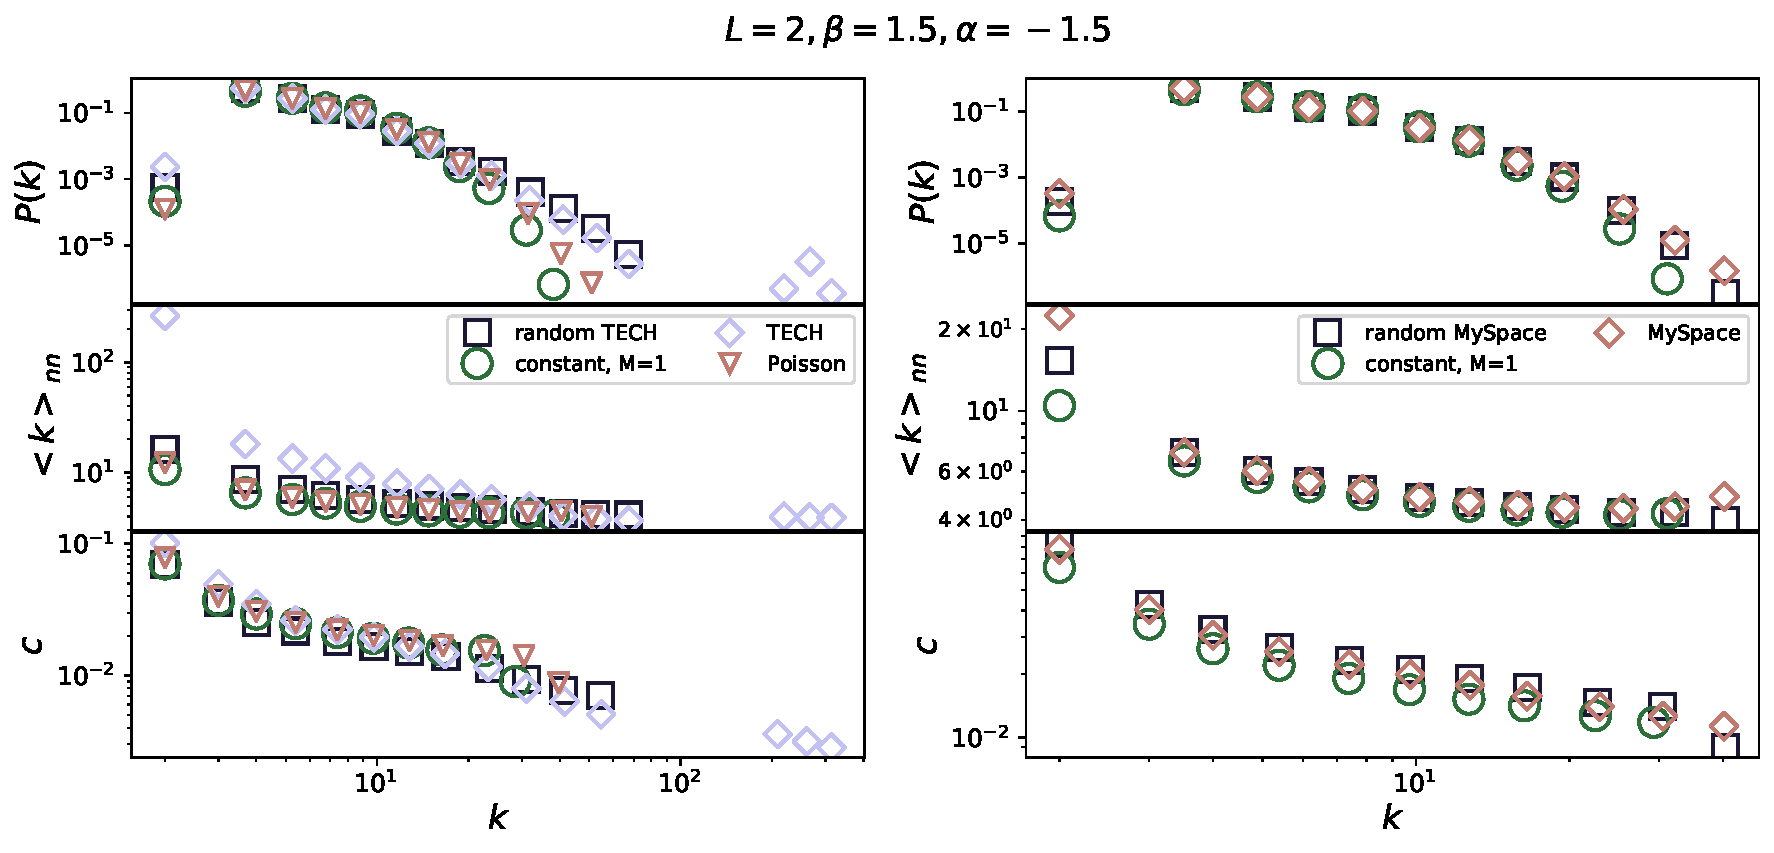
\includegraphics[width=0.7\textwidth]{Figures/b3.pdf}
	\caption{Degree distribution, the dependence of average first neighbor degree on node degree, dependence of node clustering on node degree for networks grown with different time-varying and constant signals. Model parameters have value $L=2, \alpha=-1.5$, $\beta=1.5$. The networks have stretched exponential degree distribution.}
	\label{fig:properties_se}
\end{figure}

The properties of time-varying signal do not influence the topological properties of small-world gel networks, Figure \ref{fig:properties_sw}. Here model promote existence of hubs. As this is mechanism through which the fluctuations alter the structure of evolving networks, the properties of the signal are not relevant.  


\begin{figure}[h!]
	\centering
	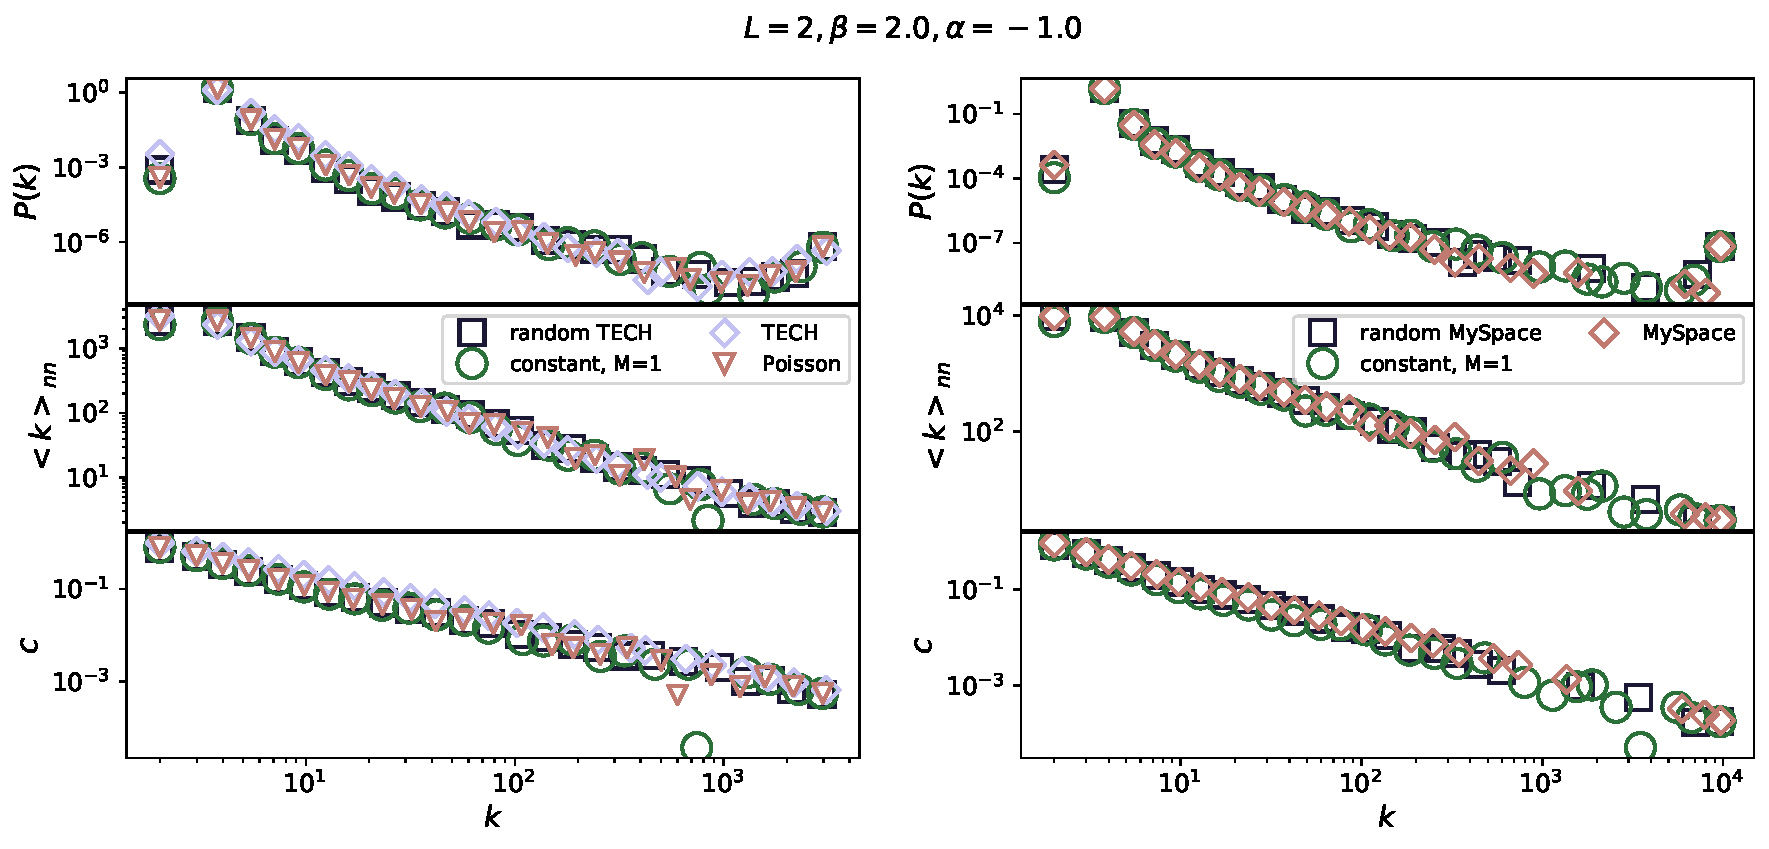
\includegraphics[width=0.7\textwidth]{Figures/b2.pdf}
	\caption{Degree distribution, the dependence of average first neighbor degree on node degree, dependence of node clustering on node degree for networks grown with different time-varying and constant signals. Model parameters have value $ L=2, \alpha=-1.0$, $\beta=2.0$. Generated networks have scale-free properties.}
	\label{fig:properties_sw}
\end{figure}

\newpage
\section{Conclusions}

We demonstrate that the resulting networks' structure depends on the features of the time-varying signal that drives their growth. The previous research \cite{mitrovic2012,mitrovic2015} indicated the possible influence of temporal fluctuations on network properties. Our results show that the temporal properties of growth signals generate networks with power-law degree distribution, non-trivial degree-degree correlations, and clustering coefficient even though the local linking rules, combined with constant growth, produce uncorrelated networks for the same values of model parameters \cite{hajra2004}. 

We observe the most substantial dissimilarity in network structure along the critical line, the values of model parameters for which we generate networks with broad degree distribution. Figure \ref{fig:dmeasure} shows that dissimilarity between networks grown with time-varying signals and ones grown with constant signals always exists along this line regardless of the features of growth signal. However, the magnitude of this dissimilarity strongly depends on these features. We observe the largest structural difference between networks grown with multifractal TECH signal and networks that evolve by adding one node in each time step. The identified value of D-measure is similar to one calculated in the comparison between sub-critical and super-critical Erd\"{o}s–R\'{e}nyi graphs \cite{tiago2} indicating the considerable structural difference between these networks. Our findings are further confirmed in figure \ref{fig:properties}(b). The networks generated with signals that have trends and long-range temporal correlations differ the most from those grown with the constant signal. Our results show that even white-noise type signals can generate networks significantly different from ones created with constant signal for low values of $\alpha^{*}$.

The value of D-measure declines fast as we move away from the critical line, figure \ref{fig:dmeasure}. The main mechanism through which the fluctuations influence the structure of evolved networks is the emergence of hubs and super hubs. For values of $\alpha<<\alpha^{*}$, the nodes attache to their immediate predecessors creating regular networks without hubs. For $\alpha \sim \alpha^{*}$ graphs have stretched exponential degree distribution with low potential for the emergence of hubs. Still, multifractal signal TECH enables the emergence of hub even for the values of parameters for which we observe networks with stretched-exponential degree distribution in the case of constant growth figure \ref{fig:properties}(a). By definition, small-world gels generated for $\alpha>\alpha^{*}$ have super-hubs \cite{hajra2004} regardless of the growth signal, and therefore the effects that fluctuations produce in the growth of networks do not come to the fore for values of model parameters in this region of $\alpha-\beta$ plane.

Evolving network models are an essential tool for understanding the evolution of social, biological, and technological networks and mechanisms that drive it \cite{boccaletti2006}. The most common assumption is that these networks evolve by adding a fixed number of nodes in each time step \cite{boccaletti2006}. So far, the focus on developing growing network models was on linking rules and how different rules lead to networks of various structural properties \cite{boccaletti2006}. Growth signals of real systems are not constant \cite{mitrovic2015,mitrovic2012}. They are multifractal, characterised with long-range correlations \cite{mitrovic2015}, trends and cycles \cite{suvakov2013}. Research on temporal networks has shown that temporal properties of edge activation in networks and their properties can affect the dynamics of the complex system \cite{holme2012}. Our results imply that modeling of social and technological networks should also include non-constant growth and that its combination with local linking rules can significantly alter the structure of generated networks.

%----------------------------------------------------------------------------------------


